\documentclass{beamer}
\usetheme{dianahep}

%
% Title definitions
%

\title{NSF $ S^2 I^2 $\\ ``Scientific Software Innovation Institute'' \\ Conceptualization}
\author{Peter Elmer - Princeton University \\
        Mike Sokoloff - University of Cincinnati \\
        Mark Neubauer - University of Illinois at Urbana-Champaign}
\date{19 May, 2016}

\begin{document}
\maketitle
%\insertframenumber/\inserttotalframenumber

%
% Presentation body
%

\setbeamertemplate{footline}[frame number]
\begin{frame}
 \frametitle{Software Challenges at the HL-LHC}

\begin{itemize}
\item The process to define the computing and analysis models for the HL-LHC era has begun in recent years, with a handful of R\&D projects exploring various topics.
\item Given the 20 year time scale and physics goals of the HL-LHC, several major software sustainability challenges exist: 
(1) the evolution of computing hardware (processors,
storage, networks) and the need to find cost-effective solutions,
(2) increased complexity of the data %%  mds (due to higher pile-up)
and/or detectors, and (3) increased sophistication of analyses required
from larger datasets.
\item In order to achieve the HL-LHC physics goals, and do so at a acceptable
cost, we need a broad vision of software and computing in the HL-LHC era and an upgrade path to realize that vision.
\item In this presentation we present one possible path to achieve this.
\end{itemize}

\end{frame}

\begin{frame}
\frametitle{NSF CIF21 Software Vision}

From \url{http://www.nsf.gov/funding/pgm_summ.jsp?pims_id=504817}
\vskip 0.15in
``NSF's vision of a Cyberinfrastructure Framework for 21st Century Science and Engineering (CIF21) identifies advancing new computational infrastructure as a priority for driving innovation in science and engineering. Innovation occurs through advances in computing facilities, scientific instruments, software environments, advanced networks, data storage capabilities, and the critically important human capital and expertise. Software is thus an integral enabler of computation, experiment and theory and a central component of the new computational infrastructure. Scientific discovery and innovation are advancing along fundamentally new pathways opened by the development of increasingly sophisticated software. Software is also directly responsible for increased scientific productivity and significant enhancement of researchers' capabilities.''

\end{frame}



%\begin{frame}
\frametitle{NSF Software Vision - Five Strategic Goals}
\fontsize{11pt}{7.2}\selectfont
%Implementing NSF's CIF21 Software Vision (NSF 12-113) is a Foundation-wide effort that includes multiple programs with the goal of nurturing, accelerating, and sustaining this critical mode of scientific progress. 
\begin{itemize}
\item {\bf Capabilities:} Support the creation and maintenance of an innovative, integrated, reliable, sustainable and accessible software ecosystem providing new capabilities that advance and accelerate scientific inquiry and application at unprecedented complexity and scale.
\item {\bf Research:} Support the foundational research necessary to continue to efficiently advance scientific software, responding to new technological, algorithmic, and scientific advances.
\item {\bf Science:} Enable transformative, interdisciplinary, collaborative, science and engineering research and education through the use of advanced software and services.
\item {\bf Education:} Empower the current and future diverse workforce of scientists and engineers equipped with essential skills to use and develop software. Further, ensure that the software and services are effectively used in both the research and education process realizing new opportunities for teaching and outreach.
\item {\bf Policy:} Transform practice through new policies for software addressing challenges of academic culture, open dissemination and use, reproducibility and trust of data/models/ simulation, curation and sustainability, and that address issues of governance, citation, stewardship, and attribution of software authorship.
\end{itemize}

\end{frame}



\begin{frame}
\frametitle{National Academies Report}

\begin{figure}[htbp]
\begin{center}
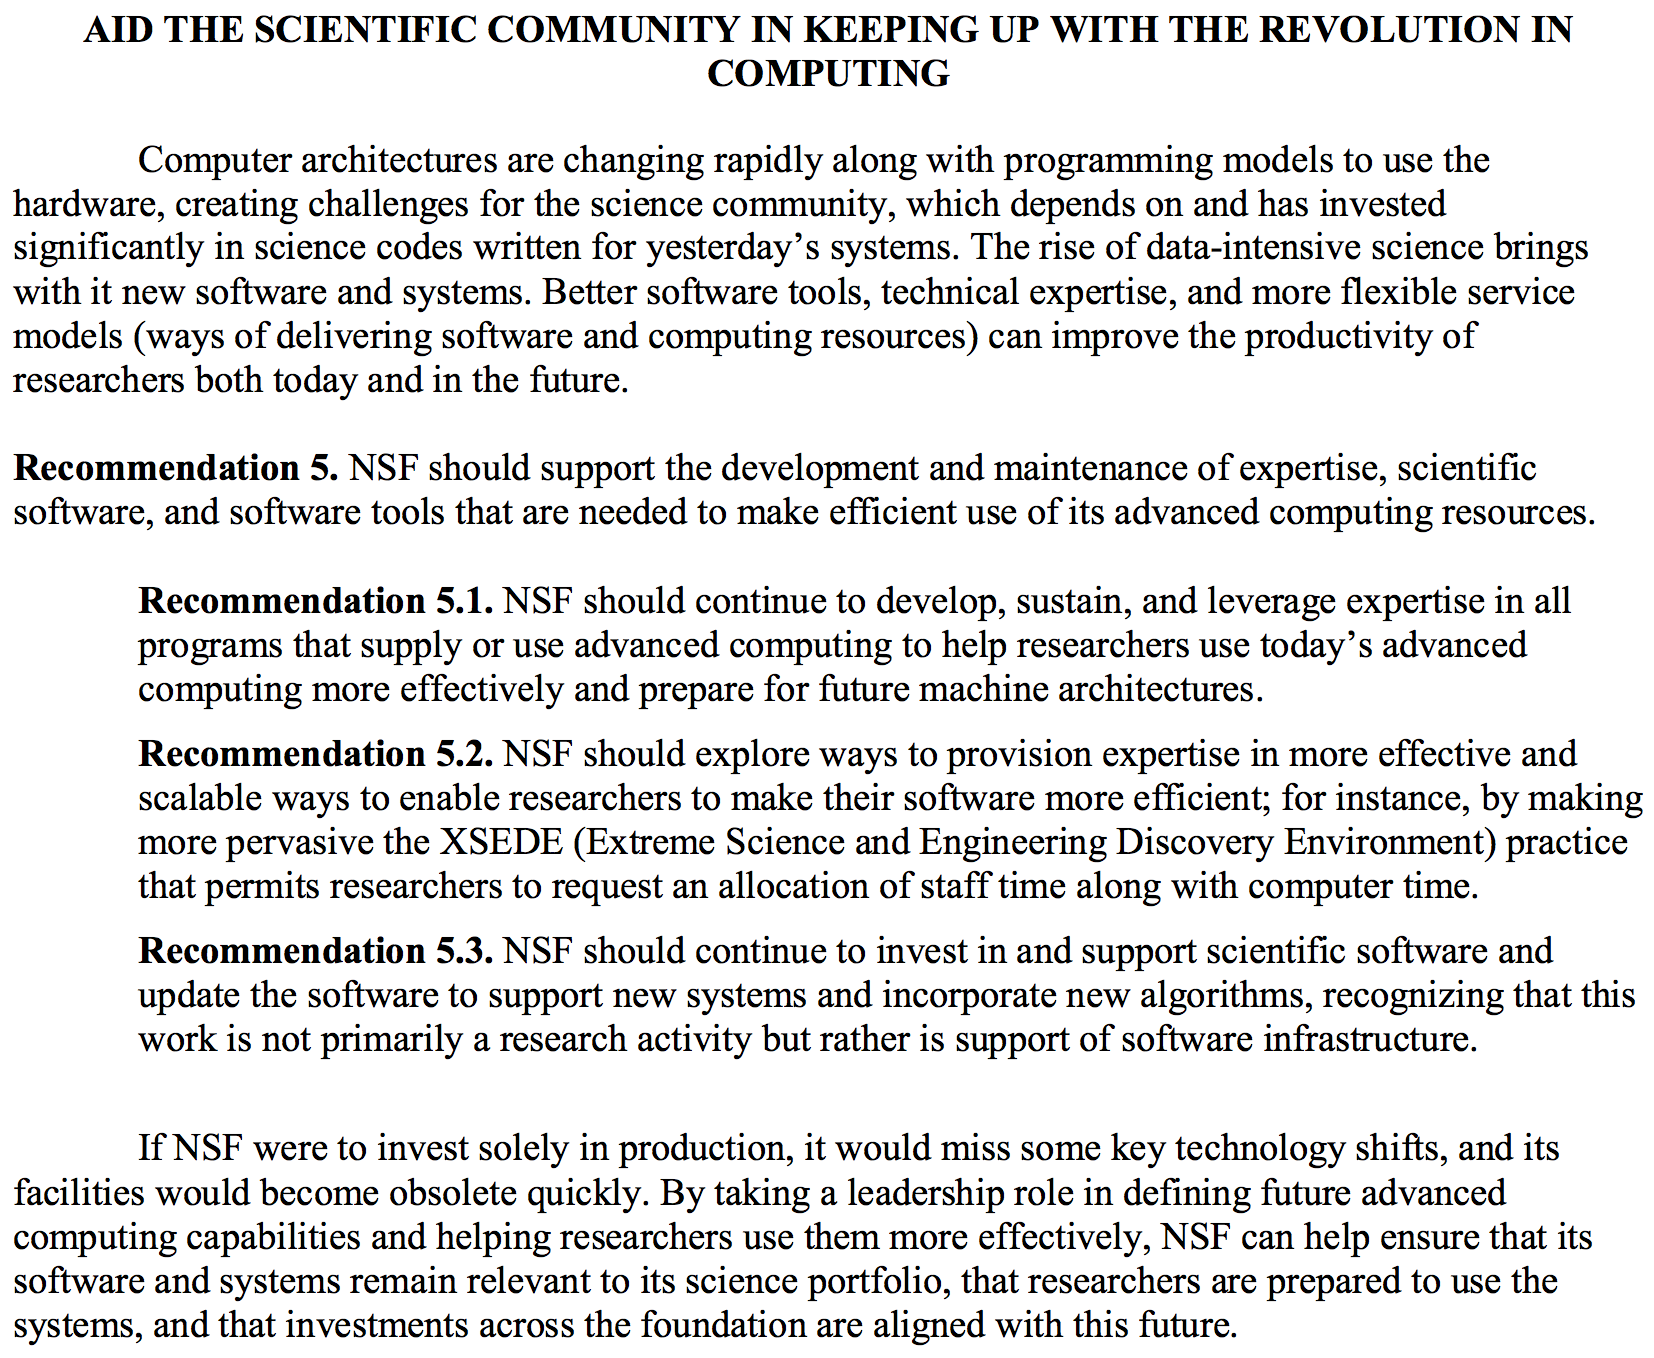
\includegraphics[width=0.65\textwidth]{images/NAS-recommendation-software.png}
%\caption{}
\label{fig:nsfsi2}
\end{center}
\end{figure}

\small{Future Directions for NSF Advanced Computing Infrastructure to Support U.S. Science and Engineering in 2017-2020 (2016)}
\end{frame}



\begin{frame}
\frametitle{Software Infrastructure for Sustained Innovation (SI2)}

\small{Implemented by NSF Division of Advanced Cyberinfrastructure (ACI), within the Directorate for Computer \& Information Science (CISE)}

\begin{figure}[htbp]
\begin{center}
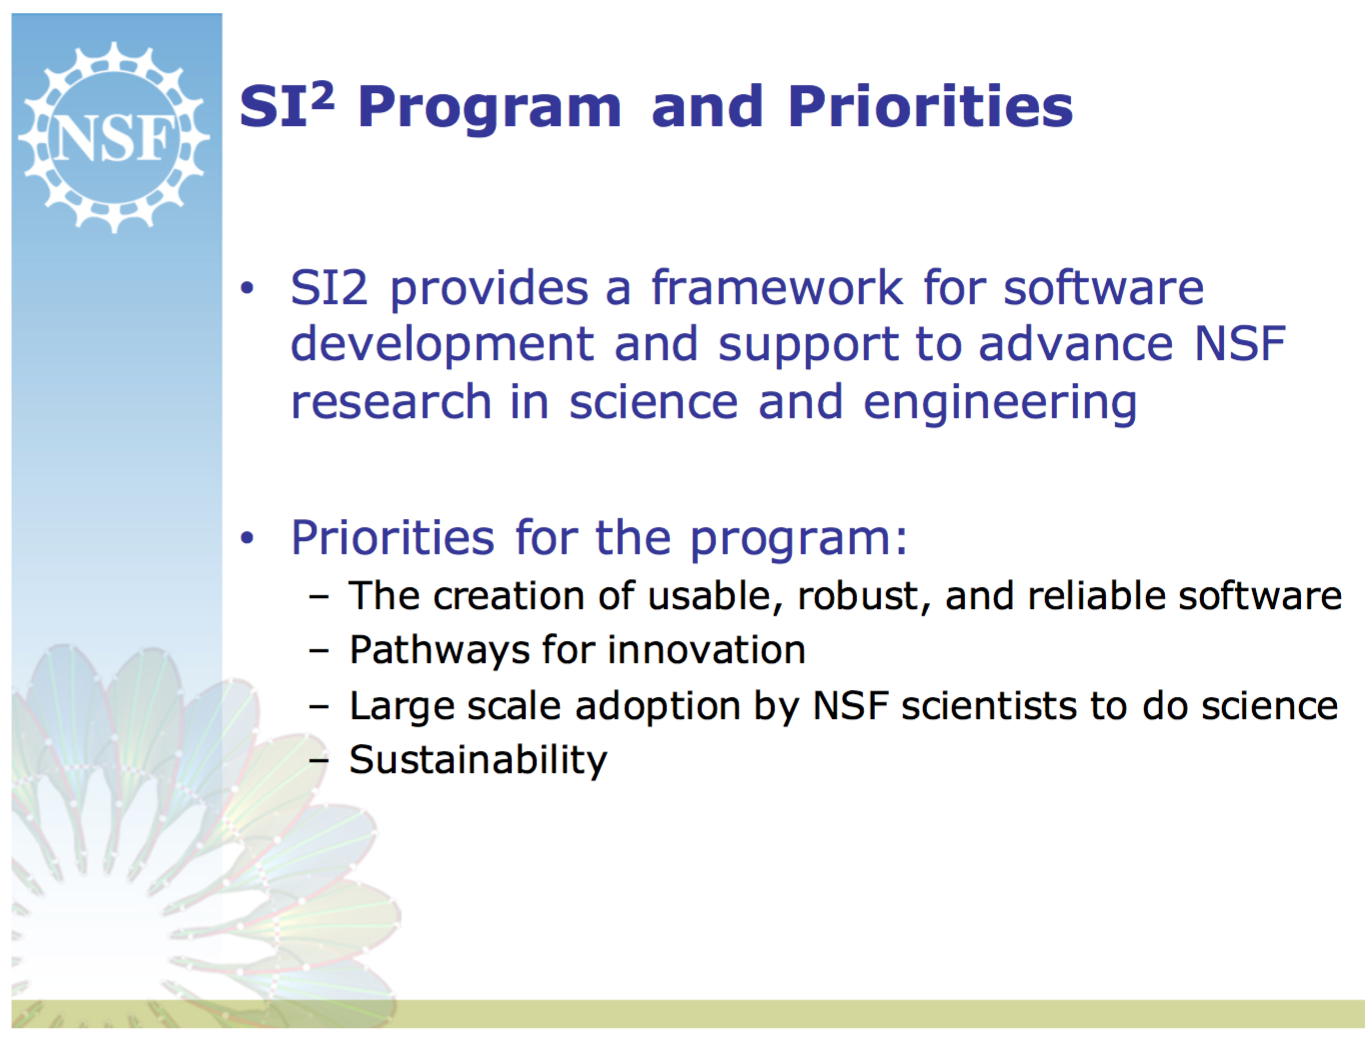
\includegraphics[width=0.7\textwidth]{images/nsf-si2-priorities.png}
%\caption{}
\label{fig:example2}
\end{center}
\end{figure}

\end{frame}



\begin{frame}
\frametitle{Software Infrastructure for Sustained Innovation (SI2)}

\begin{figure}[htbp]
\begin{center}
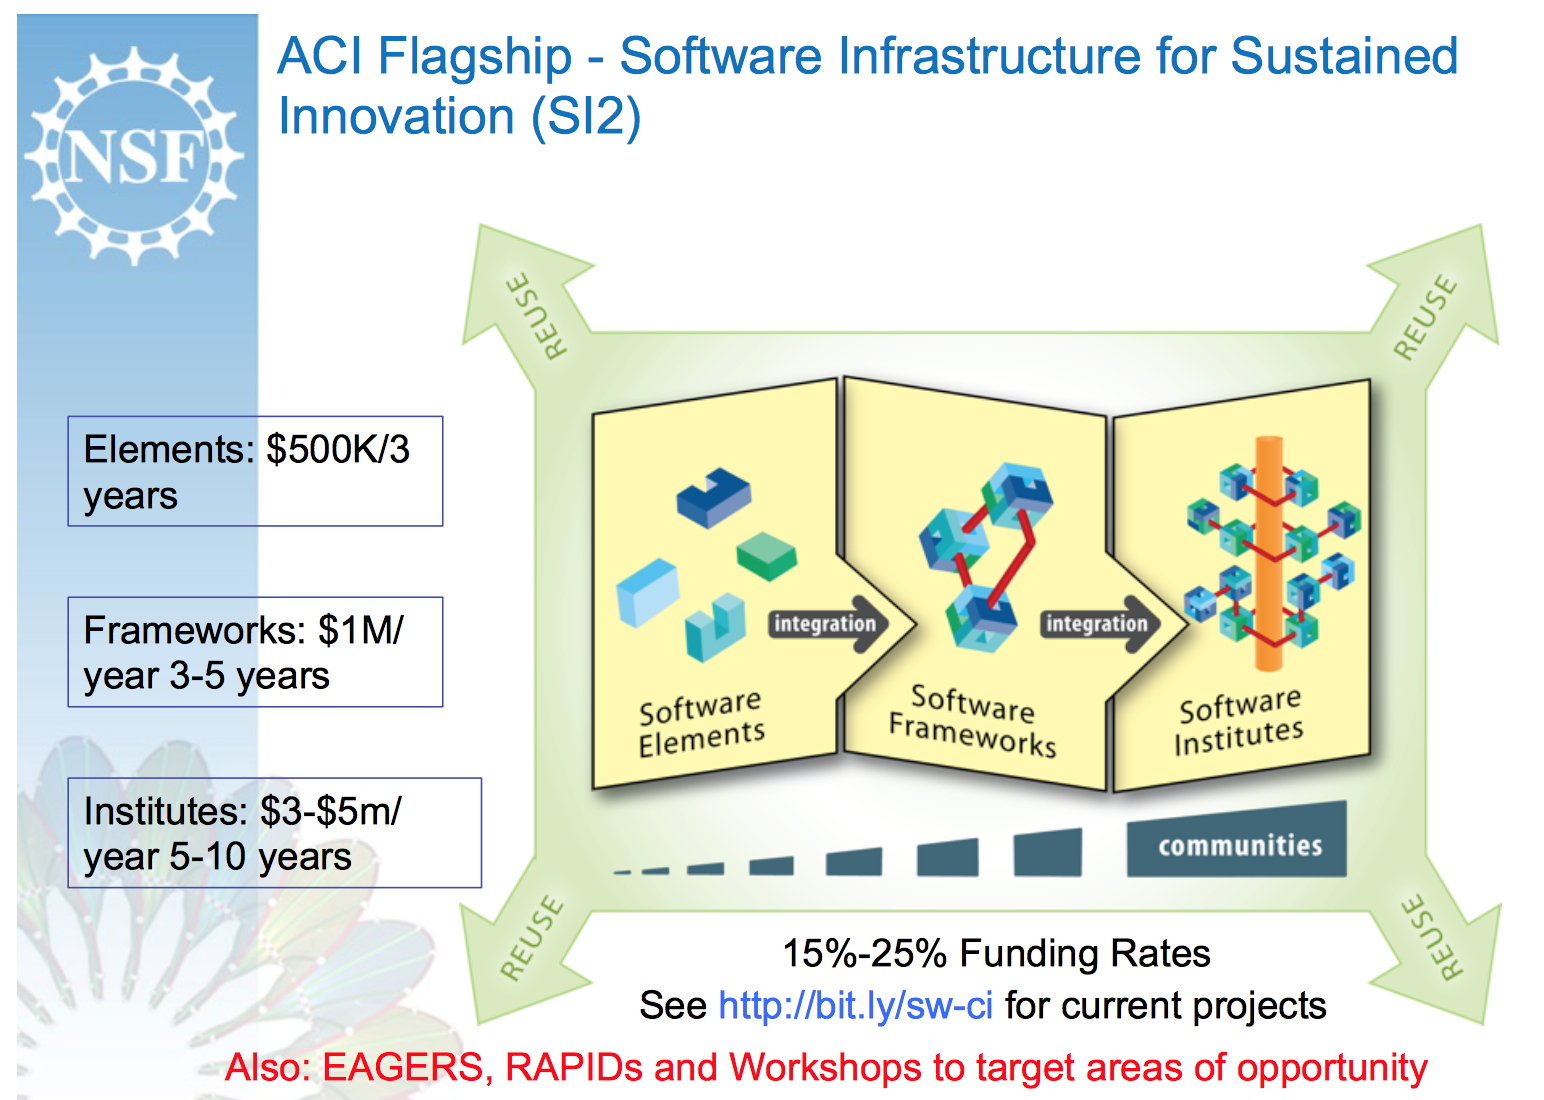
\includegraphics[width=0.75\textwidth]{images/ramnath-si2-pi-meeting-2016.png}
%\caption{}
\label{fig:nsfsi2}
\end{center}
\end{figure}

DIANA-HEP is a ``Software Framework'' (SSI).  Here we will talk about the ``Software Institute'' class of awards.

\end{frame}



\begin{frame}
\frametitle{NSF SI2 Award Classes}

The NSF SI2 program includes three classes of awards:
\begin{itemize}
\item {\bf Software Elements (SSE)} target small groups that will create and deploy robust software elements for which there is a demonstrated need that will advance one or more significant areas of science and engineering.

\item {\bf Software Frameworks (SSI)} target larger, {\em interdisciplinary} teams organized around the development and application of elements of common software infrastructure aimed at solving common research problems. These awards will result in sustainable community software frameworks serving a diverse community.

\item {\bf Scientific Software Innovation Institutes ($ S^2 I^2 $)} focus on the establishment of long-term hubs of excellence in software infrastructure and technologies, including elements and frameworks, that will serve a {\em research community of substantial size and disciplinary breadth}.
\end{itemize}

\end{frame}



\begin{frame}
\frametitle{NSF SI2-S2I2 Software Institute}

NSF SI2-S2I2 includes two subclasses of awards:
\begin{itemize}
\item \underline{Conceptualization Awards} - which are planning awards aimed at organizing an interdisciplinary community and understanding their software requirements and challenges (\$500k, 1-2 years)
\item \underline{Implementation Awards} - which will be made to implement community activities that support software infrastructure, for example, such as those developed by the conceptualization awards (\$3-5M/year, 5 years)
\item The first solicitation for implementation proposals was last June; we anticipate announcements of these awards shortly.
\item \url{http://www.nsf.gov/pubs/2015/nsf15553/nsf15553.htm}
\end{itemize}

We submitted a conceptualization proposal to NSF last August (2015):
\begin{itemize}
\item Conceptualization of an $ S^2 I^2 $ Institute for High Energy Physics
\item \url{http://cern.ch/elmer/s2i2-2015-nsf-proposal.pdf}
\end{itemize}

\end{frame}



\begin{frame}
\frametitle{$ S^2 I^2 $ Conceptualization Status}

\begin{itemize}
\item We were told a couple of months ago that the $ S^2 I^2 $ Conceptualization proposal would be recommended for funding
\item It funds a fraction of the time of P.Elmer, M.Neubauer and M.Sokoloff to organize the conceptualization activity, plus participant funds to bring people to workshops
\item We have not yet received the awards for this $ S^2 I^2 $ Conceptualization, but we are nonetheless beginning some initial broader discussions about how to actually organize it in practice (in this meeting and others)
\end{itemize}

\end{frame}



\begin{frame}
\frametitle{$ S^2 I^2 $ Conceptualization Awards}

$ S^2 I^2 $ Conceptualization Awards are {\em planning} awards aimed at organizing an interdisciplinary community and understanding their software requirements and challenges. 
Example activities that may be undertaken as part of this award include focused workshops, special sessions at professional meetings, sandpits, focus groups, etc. 
%These awards will typically be 1 year in duration. 
\vskip 0.12in
The product of a conceptualization award will be a {\bf Strategic Plan} for enabling science and education through a sustained software infrastructure that will be freely available to the community. 
\vskip 0.12in
The Strategic Plan resulting from the conceptualization phase is expected to serve as the conceptual design upon which a subsequent $ S^2 I^2 $ Implementation proposal could be based.
\vskip 0.12in
Because an NSF effort cannot stand in isolation to DOE and international efforts, the process we proposed delivers also a broader {\bf Community White Paper}.

\end{frame}



\begin{frame}
\frametitle{$ S^2 I^2 $ Conceptualization - Goals for Strategic Plan}
\fontsize{11pt}{7.2}\selectfont

%An $ S^2 I^2 $ Conceptualization Awards will produce a {\bf strategic plan} which addresses the following elements:

(1) the science community and the specific grand challenge research questions that the $ S^2 I^2 $ will support; \\
(2) specific software elements and frameworks that are relevant to the community, the sustainability challenges that need to be addressed, and why addressing these challenges will be transformative; \\
(3) appropriate software architectures and lifecycle processes, development, testing and deployment methodologies, validation and verification processes, end usability and interface considerations, and required infrastructure and technologies; \\
(4) the required organizational, personnel and management structures and operational processes; \\
(5) the requirements and necessary mechanisms for human resource development, including integration of education and training, mentoring of students, postdoctoral fellows as well as software professionals, and proactively addressing diversity and broadening participation; \\
(6) potential approaches for long-term sustainability of the software institute as well as the software; and \\
(7) potential risks including risks associated with establishment and execution, necessary infrastructure and associated technologies, community engagement, and long-term sustainability. \\

\end{frame}



\begin{frame}
\frametitle{S2I2-HEP Strategic Plan (from our proposal)} 

This will include agency specific discussions which are not (necessarily) 
relevant to the large community; topics will include:
 \begin{itemize}
   \item
     where does the U.S.\ university community already have
     expertise and important leadership roles;
   \item
     which software elements/frameworks would provide
     the best educational/training opportunities
     for students and postdoctoral fellows;
   \item
     what  types of programs (short courses, short-term
     fellowships, long-term fellowships, etc.)
     might enhance the educational
     reach of an $ S^2 I^2 $;
   \item
     possible organizational, personnel and management
     structures and operational processes;
    \item
     how the investment in an $ S^2 I^2 $ can be judged
     and how the investment can be sustained
     to assure the scientific goals of the HL-LHC.
 \end{itemize}

\end{frame}



\begin{frame}
\frametitle{Conceptualization Process}

The idea is to hold a series of workshops over the next year to build the community roadmap. The initial straw-man proposal is:

\begin{itemize}
\item A ``kick-off'' workshop, in the fall in the U.S.
\item Several dedicated ``topical'' workshops in the {fall, winter, spring} covering software required in the various areas:
\begin{itemize}
\item Detector Simulation, Triggering, Event Reconstruction and Visualization
\item Data Access and Management, Workflow and Resource Management
\item Physics generators, Data Analysis and Interpretation, Data and Software Preservation
\end{itemize}
\item A final workshop, probably next summer (near CERN?)
\end{itemize}

These will involve the full HEP community and will be co-branded with the HEP Software Foundation (HSF). The process will also build on existing community activities when possible (e.g.\ DASPOS/DPHEP, etc.) and should be supported by dedicated working groups.

\end{frame}



\begin{frame}
\frametitle{Software Scope}
\begin{itemize}
\item Note that ``software'' here is defined very broadly, not just in terms of (for example) the scope of the US-CMS and US-Atlas S\&C Ops programs. 
\item The next 3 slides contain a list of example software areas and challenges. This is probably not comprehensive and not all will be realizable with an $ S^2 I^2 $ (but perhaps they could be within the full HEP community)
\item If the font is too small to read, see pages 9-10 in \url{http://cern.ch/elmer/s2i2-2015-nsf-proposal.pdf}
\end{itemize}

\end{frame}



\begin{frame}
\frametitle{Detector Simulation, Triggering, Event Reconstruction and Visualization} 
\scriptsize{
Challenges surrounding high pile-up simulation,
including the CPU resources needed for large statistics samples
needed to compare with data from high trigger rates, high memory
utilization, generation and handling of the large (min-bias) samples
needed to achieve accurate description of high pile-up collision
events, and a flexible simulation strategy capable of a broad
spectrum of precision in the detector response, from ``fast''
(e.g. parametric) simulation optimized for speed to full simulation
in support of precision measurements and new physics searches
(e.g. in subtle effects on event kinematics due to the presence of
virtual particles at high scale).
Software required to emulate upgraded detectors (including the
trigger system) and support determination of their optimal
configuration and calibration.
Software in support of triggering
during the HL-LHC, including algorithms for the High-level Trigger,
online tracking using GPUs and/or FPGAs, trigger steering, event
building, data ``parking'' (for offline trigger decision), and data
flow control systems. New approaches to event reconstruction, in
which the processing time depends sensitively on instantaneous
luminosity, including advanced algorithms, vectorization, and
execution concurrency and frameworks that exploit many-core
architectures. In particular, charged particle tracking is expected
to dominate the event processing time under high pile-up
conditions. Visualization tools, not only in support of upgrade
detector configurations and event displays, but also as a research
tool for data analysis, education, and outreach using modern tools
and technologies for 3D rendering, data and geometry description and
cloud environments.
}
\end{frame}



\begin{frame}
\frametitle{Data Access and Management, Workflow and
Resource Management}
\scriptsize{ 
Data handling systems that scale to the Exabyte level during the
HL-LHC era and satisfy the needs of physicists in terms of metadata
and data access, distribution, and replication. Increasing
availability of very high speed networks removes the need for CPU
and data co-location and allows for more extensive use of data
access over the wide-area network (WAN), providing failover
capabilities, global data namespaces, and caching. Event-based data
streaming as complementary to the more traditional dataset-based or
file-based data access, which is particularly important for
utilizing opportunistic cycles on HPCs, cloud resources, and campus
clusters where job eviction is frequent and stochastic. Workflow
management systems capable of handling millions of jobs running on a
large number of heterogeneous, distributed computing resources, with
capabilities including whole-node scheduling, checkpointing, job
rebrokering, and volunteer computing. Systems for measurement and
monitoring of the networking bandwidth and latency between resource
targets and the use of this information in job
brokering. Software-defined networking technologies which enable
networks to be configurable and schedulable resources for use in the
movement of data.
}

\end{frame}



\begin{frame}
\frametitle{ Physics generators, Data Analysis and Interpretation, Data and Software Preservation}
\scriptsize{ 
There are many theory challenges in the HL-LHC era, among them are
improving the precision of SM calculations, better estimation of
systematic uncertainties, and elucidation of promising new physics
signals for the experiments. Software needed to make connection
between observations and theory include matrix element generators,
calculation of higher-order QCD corrections, electroweak
corrections, parton shower modeling, parton matching schemes, and
soft gluon resummation methods. Physics generators that employ
concurrency and exploit many-core architectures will play an
important role in HL-LHC, as well better sharing of code and
processing between LHC experimenters and phenomenologists. Data
analysis frameworks that include parallelization, optimized event
I/O, data caching, and WAN-based data access. Analysis software
that employs advanced algorithms and efficiently utilizes many-core
architectures. Tools and technologies for preservation and reuse of
data and software, preservation and re-interpretation of physics
results, analysis providence and workflow ontologies, analysis
capture, and application packaging for platform abstraction. Future
software repositories and build platforms that leverage advances in
these areas and improved software modularity and quality control
that will allow a broader community of people to effectively
contribute to software in the HL-LHC era.}

\end{frame}



\begin{frame}
\frametitle{Recent NSF funded HEP S\&C projects (PIF, SI2)}
\begin{itemize}
\item In addition to DASPOS, OSG and many software projects within US-CMS and US-Atlas, etc. we have: \\
\item PIF: Any Data, Anytime, Anywhere (S.Dasu, K.Bloom, F.Wuerthwein)
\item PIF: Enabling High Energy Physics at the Information Frontier Using GPUs and Other Many/Multi-Core Architectures (M.Sokoloff)
\item PIF: Particle Tracking at High Luminosity on Heterogeneous, Parallel Processor Architectures (P.Elmer, P.Wittich, A.Yagil, F.Wuerthwein)
\item SI2-SSI: Data-Intensive Analysis for High Energy Physics (DIANA/HEP) (P.Elmer, M.Sokoloff, K.Cranmer, B.Bockelman)
\end{itemize}

\end{frame}



\begin{frame}
\frametitle{Recent NSF funded HEP S\&C projects (PIF, SI2)}
\begin{itemize}
\item SI2-SSI: Distributed Workflow Management Research and Software in Support of Science (E.Deelman, M.Livny)
\item SI2-SSE: Connecting Cyberinfrastructure with the Cooperative Computing Tools (D.Thain)
\item SI2-SSE: Enhancement and Support of DMTCP for Adaptive, Extensible Checkpoint-Restart (G.Cooperman)
\item Both this slide and the previous side are examples, there are obviously many other software activities/projects that are relevant that I am not listing here.
\end{itemize}
\end{frame}

\begin{frame}
\frametitle{Build on earlier community efforts}
\begin{itemize}
\item Snowmass Computing Frontier: Planning the Future of U.S. Particle Physics (Snowmass 2013): Chapter 9: Computing [arXiv 1401.6117], plus supporting docs and white papers.

\item \underline{Including one specific SI2-relevant support document}: Snowmass Computing Frontier: Software Development, Staffing and Training [arXiv 1311.2567]

\item Separate DOE Lab "Center for Computational Excellence" (HEP-CCE, n\'{e}e HEP-FCE) process (see hepfce.org for documents)

\item WLCG TDR/Comp. Model Update, etc.
\end{itemize}

\end{frame}



\begin{frame}
\frametitle{Community White Paper (CWP)}

\noindent A Strategic Plan for an NSF Software Institute cannot be formulated without reference to DOE and international efforts. Thus the workshops and planning will engage the larger community with the aim of writing a {\bf Community White Paper (CWP)}.
\vskip 0.15in
\noindent The CWP should describe a global vision and roadmap for R\&D for 
software and computing 
for the HL-LHC era and HEP in the 2020s; this should include discussions of 
elements that are common to
the HEP community (LHC community, etc.) as a whole and those that are specific
to the individual experiments.
It should also discuss the relationship of the common elements
to the broader scientific computing communities.

\end{frame}



\begin{frame}
\frametitle{Community White Paper (CWP)}

\begin{itemize}
  \item
    a broad overview of the grand challenge science (HL-LHC, HEP);
  \item
    how new approaches to computing and software can enable and
    radically extend the physics reach of the detectors;
  \item
    what computing and software research will be required so that
    (for example) computing and software Technical Design Reports
    can be prepared several years before Run 4 of the LHC begins;
    this will include studies of hardware and software architectures
    and life-cycle processes and costs.
   \item
    identify specific software elements and frameworks that will
    be required for the HL-LHC era which can be built and tested
    during Run 3.
   \item
     organizational issues for the common software and for
     coordinating research of common interest, even when the
     final products will be specific to individual experiments.
  \item
     software development and documentation tools for
     writing sustainable software;
%  \item identifying and mitigating potential risks
\end{itemize}


\end{frame}



\begin{frame}
\frametitle{Working groups - example questions to address}

In addition to addressing issues specific to a given topic,
each group should presumably address questions which cut across boundaries,
including:
\begin{itemize}
\item
  What are the specific challenges for the HL-LHC (IF, etc.)?
\item
  What opportunities exist to exploit new or advanced
  algorithms (e.g.\ deep learning)?
\item
  How can emerging architectures improve the bang-per-buck and what
  software evolution is needed to exploit them?
\item
  Which problems are specific to individual experiments and which
  are common to (for example) the HL-LHC experiments or to HEP
  and nuclear physics experiments
  more generally?
\item
  What is required to make common software packages sustainable?
\end{itemize}


\end{frame}



%\begin{frame}
\frametitle{Recognition/Endorsement of the CWP (and HSF)}

One important thing we will presumably need to accomplish is eventual 
recognition and endorsement of the CWP (and in some more formal sense, HSF) 
by various entities: funding agencies, labs, experiments, ICFA, etc. 
\vskip 0.15in
How do we do that?

\end{frame}



\begin{frame}
\frametitle{Discussion}
We are just now beginning this conceptualization process and it will play out over the next year or so.
\vskip 0.15in
Your comments and questions are welcome on all related topics, including:
\begin{itemize}
\item practicalities of how to organize meetings, working groups, etc. for the conceptualization process
\item thoughts regarding possible priorities, scope and specific goals for an $ S^2 I^2 $
\item thoughts regarding how an $ S^2 I^2 $ could work in practical terms
\item thoughts on how an NSF $ S^2 I^2 $ could relate to DOE and/or international efforts
\end{itemize}

\end{frame}



\end{document}


